\documentclass{ximera}
\typeout{Start loading xmPreamble.tex}%

% Extra macros loaded automatically by all documents of class 'ximera' or 'xourse'

\newcommand{\PP}{\mathbb{P}}
\newcommand{\EE}{\mathbb{E}}
\newcommand{\Var}{\mathrm{Var}}
\newcommand{\indep}[2]{\PP\left(#1 \cap #2\right) = \PP\left(#1\right) \cdot \PP\left(#2\right)}
\newcommand{\cond}[2]{\frac{\PP( #1 \cap #2)}{\PP(#2)}}
\newcommand{\pdf}{\text{probability distribution function}}

% Ximera already defines theorem-like environments:
% theorem, lemma, corollary, example, definition, etc.
% So do NOT redefine them here.

\usepackage{tikz}
\usetikzlibrary{positioning, arrows.meta}

\usepackage{multicol}
\usepackage{enumitem}
\usepackage{caption}
\usepackage{amsmath,amssymb,amsfonts}
\usepackage{mathtools}
\usepackage{graphics}
\usepackage[T1]{fontenc}
\usepackage{colortbl}
% \usepackage{fouriernc}
\usepackage{marvosym}
\usepackage{color}

\providecommand{\Lightning}{\ensuremath{\text{\sffamily\bfseries !}}}

\def\arrvline{\hfil\kern\arraycolsep\vline\kern-\arraycolsep\hfilneg}

\title{Chapter 5}
\begin{document}
\begin{abstract}
\end{abstract}
\maketitle
\section{Law of Large Numbers (LLN) and Central Limit Theorem (CLT)}

\subsection{Inequalities}
In the last section, we saw the Laplace -- deMoivre theorem, which showed that a Binomial random variable converges to a normal random variable (in the right scaling). A binomial random variable can be written as the sum of independent $\mathrm{Ber}(p)$. The main topic of this chapter will be a generalization of the Laplace -- deMoivre theorem, to random variables other than the Bernoulli. These will be called the LLN and CLT.

\begin{definition}
We say that a sequence $X_1,X_2,\ldots$ of random variables is \textit{independent and identically distributed} if they are independent and have a common distribution $X$.
\end{definition}
This occurs enough that it is abbreviated to i.i.d. For example, the setup of the Laplace -- deMoivre theorem is i.i.d. \text{Ber}$(p)$.

We'll develop some inequalities that will help with proving the LLN and the CLT. These inequalities will hold for very general random variables. 

\begin{theorem}
(Markov's inequality)

If $X$ is non--negative and $a>0$, then
$$
\PP(X > a ) \leq \frac{\EE[X]}{a}.
$$
\end{theorem}
\begin{proof}
By non--negativity, we can take the integral over $(0,\infty)$:
\begin{equation*}
\EE[X]=\int_{0}^{\infty} x f_{X}(x) d x
\end{equation*}
The integral then splits up into two pieces
\begin{align*}
\EE[X] &= \int_0^a x f_X(x)dx + \int_a^{\infty} x f_X(x) dx\\
& \geq 0 + a \int_a^{\infty} f_X(x)dx.\\
&= a \PP(X >a).
\end{align*}
\end{proof}

\begin{example}
Let $X$ be uniform on $[0,4]$. Then $\mathbb{E}[X]=2$. So we have
$$
\PP(X > 2 ) \leq \frac{\EE[X]}{2} = 1, \quad \PP(X > 3) \leq \frac{\EE[X]}{3}=0.666\ldots, \quad \PP(X > 4 ) \leq \frac{\EE[X]}{4}=0.5.
$$
The true values are
$$
\PP(X > 2 ) =0.5 , \quad \PP(X > 3) =0.25, \quad \PP(X > 4 ) =0.
$$
\end{example}

\begin{example}
If $X \sim \mathrm{Exp}(\lambda)$, we have that 
$$
\PP( X > a) \leq \frac{1}{\lambda a}.
$$
The true value is 
$$
\PP(X > a ) = e^{-\lambda a}.
$$
\end{example}

We note that these are rather weak inequalities. Their main benefit is that apply to any non--negative random variable, which will make it applicable to a large range of problems. 

\begin{theorem}
(Chebyshev's inequality)

For any random variable $X$ with variance $\sigma^2$,
$$
\PP( \vert X - \mu \vert \geq k\sigma ) \leq \frac{1}{k^2}.
$$
\end{theorem}
\begin{proof}
Set $Y=(X-\mu)^2$ and $a = (k\sigma)^2$. The random variable $Y$ is non--negative, so we can apply Markov's inequality:
$$
\mathbb{P}( Y \geq a ) \leq \frac{ \EE[Y]}{a}
$$
which in this case is
$$
\PP( (X-\mu)^2 \geq (k\sigma)^2) \leq \frac{\EE[ (X-\mu)^2]}{ (k\sigma)^2}.
$$
On the left--hand--side note that the events
$$
\{  (X-\mu)^2 \geq (k\sigma)^2  \} = \{  \vert X - \mu \vert \geq k\sigma \}
$$
are the same. On the right--hand--side, the numerator is just $\mathrm{var}(X) = \sigma^2$. So we get
$$
\PP( \vert X - \mu \vert \geq k\sigma ) \leq \frac{1}{k^2}.
$$
\end{proof}
In words: the probability of a result that's at least $k$ standard deviations from the mean must be at most $1/k^2$.

\begin{example}
Suppose $X$ is uniform on $[0,4]$. We know that $\EE[X]=2$. Use Chebyshev's inequality to bound $\PP( \vert X -2 \vert \geq 1)$.
To do this, we first note that the variance is $\sigma^2=4^2/12=4/3$. We need to set $k\sigma = 1$; this means that $\sigma = 1/k$, so $\sigma^2 = 1/k^2$. Therefore
$$
\PP( \vert X - 2 \vert > 1 ) \leq \frac{4}{3}.
$$
\end{example}

\begin{example}
Let $X \sim \mathrm{Exp}(1)$. We know that $\EE[X]=1$ and $\mathrm{Var}(X)=1$. For $c>1$, we have that
\begin{equation*}
\begin{aligned} \mathbb{P}(X \geqslant c) &=\mathbb{P}(X-1 \geqslant c-1) \\ & \leqslant \mathbb{P}(|X-1| \geqslant c-1) \\ & \leqslant \frac{1}{(c-1)^{2}} \end{aligned}
\end{equation*}
\end{example}
Note that for both of these examples, the actual bound is very weak (especially since $4/3$ is already greater than one!). The main benefit is not that the bounds are strong, but rather that the inequalities apply very generally.

\subsection{Convergence}
We've seen before convergence of CDF and MGF. 

\begin{definition}
A sequence of random variables $X_1,X_2,\ldots$ converges to a random variable $X$ in distribution if the CDFs converge:
$$
\lim_{n\rightarrow \infty} F_{X_n}(x) = F_X(x)
$$
for all $x$ where $F_X$ is continuous. Write this as $X_i \stackrel{d}{\rightarrow} X$.
\end{definition}
Note that this holds whether $X$ is discrete or continuous.

\begin{example}
Let $X_1,X_2,\ldots,$ be i.i.d. uniform random variables on $[0,1]$. Let $Y_n = \min(X_1,\ldots,X_n)$. We intuitively expect that $Y_n \rightarrow 0$ for some mode of convergence. We have that
\begin{align*}
F_{Y_n}(x) &= \PP(Y_n \leq x)\\
&= 1 - \PP(Y_n \geq x)\\
&= 1 - \PP(X_1 \geq x)\cdots \PP(X_n \geq x).
\end{align*}
This is $1-(1-x)^n$ for $x \in [0,1]$. In the other cases, it is$1-0=1$ for $x > 1$ and $1-1^n=0$ for $ x<0$. So
$$
F_{Y_{n}}(x) = 
\begin{cases}
0, \quad & x < 0,\\
1-(1-x)^n, \quad & 0 \leq x \leq 1,\\
1, \quad & x \geq 1.
\end{cases}
$$
So 
$$
\lim_{n\rightarrow \infty} F_{Y_{n}}(x) = 
\begin{cases}
0, \quad & x < 0,\\
1, \quad & x \geq 0.
\end{cases}
$$
This is also the CDF of the random variable $0$, so $Y_n\stackrel{P}{\rightarrow} 0$.
\end{example}

\begin{definition}
A sequence of random variables $X_1,X_2,\ldots$ converges to a random variable $X$ in probability if
$$
\lim_{n\rightarrow \infty} \PP( \vert X_n - X\vert > \epsilon) = 0 \text{ for all } \epsilon >0.
$$ 
We write this as $X_i \stackrel{P}{\rightarrow} X$.
\end{definition}

\begin{example}
Let $X_1,X_2,\ldots,$ be i.i.d. uniform random variables on $[0,1]$. Let $Y_n = \min(X_1,\ldots,X_n)$. We intuitively expect that $Y_n \rightarrow 0$ for some mode of convergence. Indeed, 
$$
\PP( \vert Y_n - 0 \vert > \epsilon) = \mathbb{P}(X_1 > \epsilon) \cdots \mathbb{P}(X_n > \epsilon) ,
$$
which equals $(1-\epsilon)^n$. So for every $\epsilon>0$,
$$
\lim_{n\rightarrow \infty} \PP( \vert Y_n - 0 \vert > \epsilon) = 0.
$$
Therefore $Y_n \stackrel{P}{\rightarrow} 0$.
\end{example}

In the two examples above, $Y_n$ converges to $0$ both in distribution and in probability. There is, however, a key difference between the two modes of convergence. Convergence in probability requires the random variables to be defined on the same probability space $\Omega$, but this is not the case for convergence in distribution. This is reflected in the next example:

\begin{example}\label{DiPr}
(Convergence in distribution does \textit{not} imply convergence in probability). Suppose that Texas A\&M and Georgia play infinitely many football games. Assume that there is a 50-50 chance of either team winning. Denote each Texas A\&M win with a ``T'' and each Georgia in with a ``G''; so $\Omega = \{T,G\}^{\times \infty}$. Define a sequence of random variables by 
$$
X_{k}
 = 
 \begin{cases}
 1, \text{ if game number } k \text{ is an Aggie win},\\
 0, \text{ if game number } k \text{ is an Aggie loss}.
 \end{cases}
$$
Each $X_k$ is a $\textrm{Ber}(1/2)$, so $X_k$ converges to a $\textrm{Ber}(1/2)$ in distribution. However, $X_k$ will randomly switch between $0$ and $1$, so $\PP( \vert X_k - X\vert >\epsilon)$ will randomly take values $1$. Therefore, it can't converge to $0$. 

\noindent [Personally, I call it: ``you can please everybody half the time, but you can't please everybody all the time.'']
\end{example}

However, we do have:
\begin{theorem}
If $X_n \stackrel{P}{\rightarrow} X$, then $X_n \stackrel{d}{\rightarrow} X$. 
\end{theorem}
\begin{proof}
Fix $a \in \mathbb{R}$ where $F_X(a)$ is continuous. We want to show that $F_{X_n}(a) = \PP(X_n \leq a)$ converges to $F_X(a) = \PP(X \leq a)$. For any fixed $\epsilon >0$, we can write
$$
\{X_n \leq a\} = \{X_n \leq a, X \leq a + \epsilon\} \cup \{X_n \leq a, X > a + \epsilon\} ,
$$
and notice this is a disjoint union. Therefore, 
\begin{equation*}
\mathbb{P}\left(X_{n} \leqslant a\right)=\mathbb{P}\left(X_{n} \leqslant a, X \leqslant a+\varepsilon\right)+\mathbb{P}\left(X_{n} \leq a, X>a+\varepsilon\right)
\end{equation*}
The idea is that if $X_n$ is approximately $X$, then the two events $\{X_n \leq a\}$ and $\{X \leq a + \epsilon\}$ should have very high overlap. On the other hand, the two events $\{X_n \leq a\}$ and $\{X > a + \epsilon\}$ should have very low overlap, and the probability that both happen should be close to $0$. And indeed, 
$$
\{X_n \leq a, X > a + \epsilon\} \subseteq \{ X_n < X - \epsilon\} \subseteq \{ \vert X_n - X \vert > \epsilon\}.
$$
The first term can be bounded by 
\begin{align*}
\mathbb{P}\left(X_{n} \leqslant a, X \leqslant a+\varepsilon\right) &= \mathbb{P}\left(X_{n} \leq a | X \leqslant a+\varepsilon\right) \mathbb{P}(X \leqslant a+\varepsilon)\\
&\leq \mathbb{P}(X \leq a + \epsilon).
\end{align*}
Combining the last two inequalities, we have that
$$
\PP(X_n \leq a ) \leq  \mathbb{P}(X \leq a + \epsilon) + \PP(\vert X_n - X \vert > \epsilon).
$$
Or in other words, 
$$
F_{X_n}(a) \leq F_{X}(a+\varepsilon)+\mathbb{P}\left(\left|X_{n}-X\right|>\varepsilon\right)
$$
Similarly, by swapping $X$ and $X_n$ and replacing $a$ with $a-\epsilon$,
$$
F_{X}(a-\varepsilon) \leqslant F_{X_{n}}(a)+\mathbb{P}\left(\left|X_{n}-x\right|>\varepsilon\right).
$$
Therefore, the last two inequalities tell us that
$$
 F_{X}(a-\varepsilon)-\mathbb{P}\left(\left|X_{n}-X\right|>\varepsilon\right) \leqslant F_{X_{n}}(a) \leqslant F_{X}(a+\varepsilon) +\mathbb{P}\left(\left|X_{n}-X\right|>\varepsilon\right) 
$$
Taking $n\rightarrow\infty$, and using convergence in probability, yields
$$
F_{X}(a-\varepsilon) \leq \lim_{n\rightarrow \infty}F_{X_{n}}(a) \leq F_{X}(a+\varepsilon) .
$$
Now take $\epsilon\rightarrow 0$. Since $F_X$ is continuous at $a$, the sandwich theorem implies that
$$
\lim_{n\rightarrow \infty}F_{X_{n}}(a)  = F_X(a).
$$
\end{proof}

Although convergence in distribution does not imply convergence in probability, we do have that convergence in distribution to a constant does imply convergence in probability. Think back to Example \ref{DiPr}. You can imagine instead a game where the match is always fixed, so there's only one outcome. You won't have the possibility of the variables $X_n$ alternating between $0$ and $1$, so the previous example just won't occur. 

\begin{proposition}
If $X_n \stackrel{d}{\rightarrow} c$, then $X_n \stackrel{P}{\rightarrow} c$. 
\end{proposition}
\begin{proof}
The CDF of the constant random variable $c$ is given by 
$$
F_{c}(x)=\left\{\begin{array}{ll}{1,} & {x \geqslant c} \\ {0,} & {x<c}\end{array}\right.
$$
Because we know convergence in probability, 
$$
\begin{array}{l}{\lim _{n \rightarrow \infty} F_{X_{n}}(c-\varepsilon)=0} \\ {\lim _{n \rightarrow \infty} F_{X_{n}}(c+\varepsilon)=1}\end{array}
$$
So
$$
\begin{array}{l}{\lim _{n \rightarrow \infty} \mathbb{P}\left(\left|X_{n}-c\right|>\varepsilon\right)} \\ {\quad=\lim _{n \rightarrow \infty}\left[\mathbb{P}\left(X_{n} \leqslant c-\varepsilon\right)+\mathbb{P}\left(X_{n} \geqslant c+\varepsilon\right)\right]} \\ {\quad=\lim _{n \rightarrow \infty}\left[F_{X_{n}}(c-\varepsilon)+1-F_{X_{n}}(c+\epsilon)\right]} \\ {\quad=0+1-1} \\ {\quad=0}\end{array}.
$$
\end{proof}

\subsection{Law of Large Numbers}
\begin{theorem} (Weak LLN)
Let $X_1,X_2,\ldots$ be a sequence if i.i.d. random variables. Set $\mu = \mathbb{E}[X_i]$ and $\sigma^2 = \mathrm{Var}(X_i)$, and assume both are finite. Then 
$$
\frac{X_1 + \ldots + X_n}{n} \stackrel{P}{\rightarrow} \mu.
$$
\end{theorem}
\begin{proof}
Let $S_n$ be the random variable
$$
S_n = \frac{X_1 + \ldots + X_n}{n}.
$$ 
We want to show that for every $\epsilon >0$,
$$
\lim_{n\rightarrow \infty} \PP( \vert S_n - \mu \vert > \epsilon)=0,
$$
since this is the definition of convergence in probability. We will use Chebyshev's inequality. To do this, we need to know the mean and variance of $S_n$.

By linearity $\EE[S_n]=\mu$ and by independence, 
\begin{align*}
\Var\left( S_n \right) &= \Var\left( \frac{X_1}{n} \right)  + \ldots + \Var\left( \frac{X_n}{n} \right) \\
&= n^{-2}\sigma^2 + \ldots + n^{-2}\sigma^2 \\
&= n^{-1} \sigma^2.
\end{align*}
Thus, Chebyshev's inequality says that
$$
\PP( | S_n - \mu| > kn^{-1/2}\sigma) \leq \frac{1}{k^2}.
$$
Pick $k$ such that $\epsilon = kn^{-1/2}\sigma$. Then
$$
\PP( \vert S_n - \mu \vert > \epsilon) \leq \frac{\sigma^2}{\epsilon^2 n}.
$$
So 
$$
\lim_{n\rightarrow \infty} \PP( \vert S_n - \mu \vert > \epsilon)=0,
$$
as needed.
\end{proof}

\begin{example}
(An example with infinite expectation)
Let the Cauchy distribution of parameter $\gamma$ be the continuous random variable with PDF
$$
f_X(x) = \frac{1}{\pi } \frac{\gamma}{\gamma^2 + x^2}.
$$
First note that using the $u$--substitution $u=\gamma^2 + x^2$, and $du=2xdx$,
\begin{align*}
\mathbb{E}[X] &= \int_{-\infty}^{\infty} \frac{1}{\pi } \frac{\gamma x}{\gamma^2 + x^2} dx \\
&= 2 \int_0^{\infty} \frac{1}{\pi  } \frac{\gamma du}{2u}\\
&= \frac{\gamma}{\pi} \ln u \vert_{0}^{\infty}, 
\end{align*}
which diverges. So the mean is not fiinite.

Suppose $X$ and $Y$ are i.i.d Cauchy distributions with parameter $1$. By convolution, the PDF of $Z=X+Y$ is
$$
f_Z(z) = \int_{-\infty}^{\infty} \frac{1}{\pi} \frac{1}{1 + x^2} \frac{1}{\pi}  \frac{1}{1 + (z-x)^2} .
$$
With some work (or with a computer),
$$
f_Z(z) = \frac{1}{\pi} \frac{2}{z^2+4}.
$$
Therefore, by proposition 1.1 of the chapter 4 notes, the PDF of $Z/2 = (X+Y)/2$ is
$$
f_{Z/2}(z) = 2 f_Z(2z) = \frac{1}{\pi} \frac{1}{1+x^2}.
$$

So if $X_i$ is an i.i.d. sequence of Cauchy distributions, we don't have that $(X_1 + \ldots X_n)/n$ converges to a constant. In fact, $(X_1 + \ldots X_n)/n$ has the same distribution as $X_1$ for every $n$.
\end{example}

\begin{example}
(Gambler's fallacy).

A gambler at a roulette table has been betting on red. The probability of each win is $18/38$ (there are 18 red slots, 18 black slots, and two green slots). He's lost five straight. He reasons to himself ``well, I'm supposed to win $18/38$ of the time in the long run, so I'm due for a win!'' This rationale is incorrect: the LLN says that he'll win $18/38$ of the time even with independent random variables, not that later outcomes will balance previous outcomes. 
\end{example}

There is also a strong LLN, using a stronger mode of convergence. 
\begin{definition}
A sequence of random variables $X_1,X_2,X_3,\ldots$ converges to $X$ \textit{almost surely} if
$$
\PP( \lim_{n\rightarrow \infty} X_n = X)=1.
$$
We write $X_n \stackrel{a.s.}{\rightarrow} X$.
\end{definition}

\begin{definition}
If $E_1,E_2,E_3,\ldots$ are an infinite sequence of events, then the event that infinitely many of them occur is called $\{E_n \text{ i.o.}\}$.
\end{definition}

The connection between almost sure convergence and events occurring infinitely often is as follows. Define $E_n^{(\epsilon)}$ to be the event
$$
E_n^{(\epsilon)} = \{ \vert X_n - X\vert> \epsilon\}.
$$
Then 
$$
\{ \lim_{n\rightarrow \infty} X_n \neq X \} = \bigcup_{\epsilon >0} \{E_n^{(\epsilon)} \text{ i.o. } \}.
$$
So one way to show almost sure convergence is if $\{E_n^{(\epsilon)} \text{ i.o. } \}$ has probability $0$ for all $\epsilon>0$. Which leads to the question: when is $\PP(\{E_n \text{ i.o.}\})=0$? The next lemma gives a sufficient condition:

\begin{lemma} (Borel--Cantelli)
Suppose $E_1,E_2,\ldots$ are events such that
$$
\sum_{i=n}^{\infty} \PP(E_n) < \infty.
$$
Then 
$$
\mathbb{P}(E_n\   \text{i.o.}) = 0. 
$$
\end{lemma}
\begin{proof}
Let $X_n$ be the Bernoulli random variable defined by 
$$
X_n 
= 
\begin{cases}
1, \text{ if } E_n \text{ occurs},\\
0, \text{ if } E_n \text{ does not occur}.
\end{cases}
$$
Then $X= X_1 + X_2 + \ldots$ is the number of events $E_1,E_2,\ldots$ that occur. 

We have that $\EE[X_n]= \PP(E_n)$ and by assumption,
\begin{align*}
\EE[X] &= \sum_{n=1}^{\infty}\EE[X_n]\\
&=\sum_{i=n}^{\infty} \PP(E_n) < \infty.
\end{align*}
So by Markov's inequality,
$$
\PP(X > a ) \leq \frac{\EE[X]}{a}.
$$
Taking $a\rightarrow \infty$,
$$
\PP(E_n \text{ i.o.}) = \PP(X = \infty)=0.
$$
\end{proof}

\begin{theorem}
(Strong LLN)
Let $X_1,X_2,\ldots$ be i.i.d. random variables with mean $\mu$ and variance $\sigma^2$, assumed to be finite. Then
$$
\frac{X_1 + \ldots + X_n}{n} \stackrel{a.s.}{\rightarrow} \mu.
$$
\end{theorem}
\begin{proof} (sketch)
Let $S_n$ be the random variable
$$
S_n = \frac{X_1 + \ldots + X_n}{n}.
$$ 
We saw before that 
$$
\mathbb{P}\left(\left|S_{n}-\mu\right|>\varepsilon\right) \leqslant \frac{\sigma^{2}}{\varepsilon^{2} n}.
$$
By the Borel--Cantelli Lemma,
$$
S_{n^2} \stackrel{a.s.}{\rightarrow} \mu,
$$
because $\sum_{n=1}^{\infty} 1/n^2 <\infty$. The proof is completed with a bound on 
$$
\vert S_k - S_{n^2}\vert
$$
for $ n \leq k \leq (n+1)^2$.
\end{proof}

The strong LLN (almost sure convergence) implies the weak LLN (convergence in probability). This holds more generally:

\begin{theorem}
If $X_n\rightarrow X$ almost surely, then $X_n \rightarrow X$ in probability.
\end{theorem}
\begin{proof}
Let $$\mathcal{O} = \{lim_{n\rightarrow\infty} X_n \neq X\}.$$ 
By the definition of almost sure convergence, $\PP(\mathcal{O})=0$. Now fix $\epsilon>0$ again define the event
$$
E_n^{(\epsilon)} = \{ \vert X_n - X\vert> \epsilon\}.
$$
Set
$$
\mathcal{E}_n^{(\epsilon)} = E_n^{(\epsilon)} \cup E_{n+1}^{(\epsilon)} \cup \cdots,
$$
and define
$$
\mathcal{E}_{\infty}^{(\epsilon)} = \mathcal{E}_1^{(\epsilon)} \cap \mathcal{E}_2^{(\epsilon)} \cap \cdots.
$$
By the definition of limits, 
$$
\mathcal{E}_{\infty}^{(\epsilon)} \subseteq \mathcal{O}
$$
for every $\epsilon>0$. And since $\mathcal{O}$ has probability $0$, then so does $\mathcal{E}_{\infty}^{(\epsilon)} $. By the continuity of probability (see homework assignment),
$$
\lim_{n\rightarrow \infty} \PP(\mathcal{E}_{n}^{(\epsilon)} ) =0.
$$
Therefore
$$
\lim_{n\rightarrow \infty} \PP(E_n^{(\epsilon)} ) \leq \lim_{n\rightarrow \infty} \PP(\mathcal{E}_{n}^{(\epsilon)} ) = 0,
$$
which is the definition of convergence in probability.
\end{proof}

\begin{example}
(Convergence in probability does not imply convergence almost surely. )
Consider the ``sliding bump.'' Let $\Omega$ be the interval $[0,1]$ and let $\mathbb{P}$ be uniform on $\Omega$. Define the sequence of random variables $X_1,X_2,X_3,\ldots$ by 
$$
X_1(\omega) 
= 
\begin{cases}
1, & \text{ if } \omega \in [0,1/2] \\
0, & \text{ else }.
\end{cases}
\quad \quad \quad 
X_2(\omega) 
= 
\begin{cases}
1, & \text{ if } \omega \in [1/2,1] \\
0, & \text{ else }.
\end{cases}
$$
$$
X_3(\omega) 
= 
\begin{cases}
1, & \text{ if } \omega \in [0,1/3] \\
0, & \text{ else }.
\end{cases}
\quad \quad \quad 
X_4(\omega) 
= 
\begin{cases}
1, & \text{ if } \omega \in [1/3,2/3] \\
0, & \text{ else }.
\end{cases}
\quad \quad \quad 
X_5(\omega) 
= 
\begin{cases}
1, & \text{ if } \omega \in [2/3,1] \\
0, & \text{ else }.
\end{cases}
$$
\small
$$
X_6(\omega) 
= 
\begin{cases}
1, & \text{ if } \omega \in [0,\tfrac{1}{4}] \\
0, & \text{ else }.
\end{cases}
\quad   
X_7(\omega) 
= 
\begin{cases}
1, & \text{ if } \omega \in [\tfrac{1}{4},\tfrac{1}{2}] \\
0, & \text{ else }.
\end{cases}
\quad   
X_8(\omega) 
= 
\begin{cases}
1, & \text{ if } \omega \in [\tfrac{1}{2},\tfrac{3}{4}] \\
0, & \text{ else }.
\end{cases}
\quad
X_9(\omega) 
= 
\begin{cases}
1, & \text{ if } \omega \in [\tfrac{3}{4},1] \\
0, & \text{ else }.
\end{cases}
$$
\normalsize
and so forth. A visual representation is below:

\begin{center}
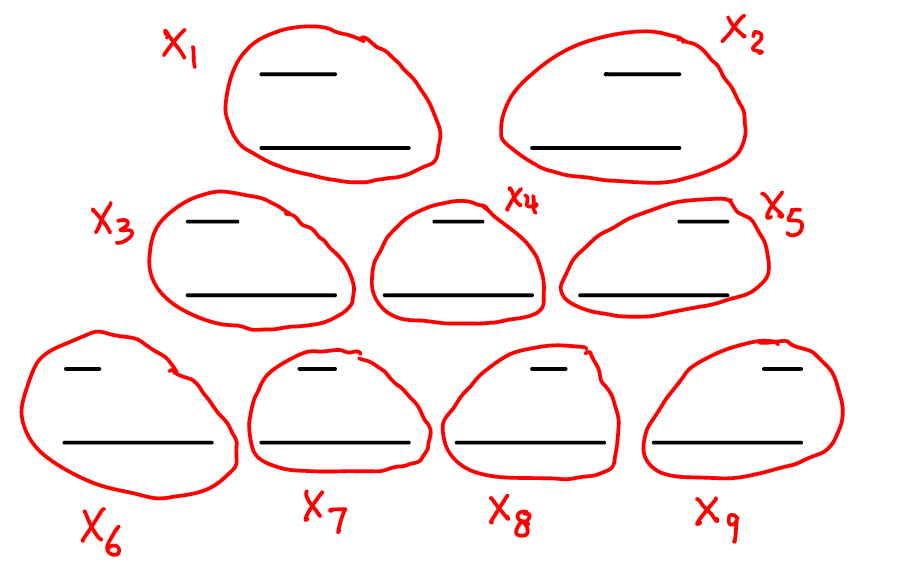
\includegraphics[height=7cm]{SlidingBump.png}
\end{center}

The quantity $\PP(\{\vert X_n - 0\vert >\epsilon\})$ takes the values $1/2,1/2,1/3,1/3,1/3,1/4,1/4,1/4,1/4,\ldots$, so it converges to $0$. Thus $X_n$ converges to $0$ in probability. 
However, for every $\omega$ in the sample space $\Omega$, $X_n(\omega)$ will be equal to $1$ infinitely often. So the set
$$
\{\lim_{n\rightarrow\infty} X_n = X\}
$$
has probability $0$, rather than probability $1$. This means that $X_n$ does not converges to $0$ almost surely.

\end{example}

\subsection{Central Limit Theorem}

We saw before in the Laplace--deMoivre theorem convergence of MGFs. We see how this relates to convergence in distribution:
\begin{theorem}
Let $X_n$ be random variables with MGF $M_{X_n}$ and $X$ be a random variable with MGF $M_X$. 
If $M_{X_n}(s) \rightarrow M_X(s)$ for all $s$ in an interval around $0$, then $X_n\rightarrow X$ in distribution.
\end{theorem}
\begin{theorem}
(Central Limit Theorem)
Let $X_n$ be i.i.d. random variables with mean $\mu$ and variance $\sigma^2$. Set 
$$
S_n = \frac{X_1 + \ldots + X_n}{n}. 
$$
Then
$$
\sigma^{-1} \sqrt{n}(S_n - \mu) \stackrel{d}{\rightarrow} \mathcal{N}(0,1).
$$
\end{theorem}
\begin{proof}
Let $M(s)$ be the MGF of $X_i - \mu$. Because the $X_i$ are identically distributed, $M(s)$ does not depend on $i$. Let
\begin{align*}
Z_n &= \sigma^{-1} \sqrt{n}(S_n - \mu)  \\
&= \frac{1}{\sigma \sqrt{n}}( (X_1 - \mu) + \ldots + (X_n- \mu))\\
&= \frac{X_1-\mu}{\sigma \sqrt{n}} + \ldots + \frac{X_n - \mu}{\sigma \sqrt{n}}.
\end{align*}
By independence and by (1) from p.10 of the chapter 4 notes, 
$$
M_{Z_n}(s) = \left[ M\left( \frac{s}{\sigma \sqrt{n}}\right)\right]^n.
$$ 
So by Levy's continuity theorem, we just need to show
$$
\lim_{n\rightarrow \infty} M_{Z_n}(s) = \lim_{n\rightarrow\infty} \left[ M\left( \frac{s}{\sigma \sqrt{n}}\right)\right]^n = e^{s^2/2}.
$$
Or equivalently, by taking natural log of both sides,
$$
\lim _{n \rightarrow \infty} n \ln M\left(\frac{s}{\sigma \sqrt{n}}\right)=\frac{s^{2}}{2}
$$
Setting $m=n^{-1/2}$, we have that
$$
\lim _{n \rightarrow \infty} n \ln M\left(\frac{s}{\sigma \sqrt{n}}\right)=
\lim _{m \rightarrow 0} \frac{\ln {M}\left(s{m} / \sigma\right)}{m^{2}}
$$
By L'Hopital's rule, 
$$
\lim _{m \rightarrow 0} \frac{\ln {M}\left(s{m} / \sigma\right)}{m^{2}} = \frac{s}{2 \sigma} \lim_{m \rightarrow 0} \frac{M^{\prime}\left(s{m} / \sigma\right)}{m M\left(sm / \sigma\right)}.
$$
Using L'Hopital again, we get
$$
\frac{s}{2\sigma} \lim_{m\rightarrow\infty} \frac{M''(sm/\sigma) (s/\sigma)}{M(sm/\sigma) + m M'(sm\sigma)(s/\sigma)}.
$$
And now we can just plug in $m=0$ to get
$$
\frac{s^2}{2\sigma^2} \frac{ M''(0)}{M(0)}.
$$
Finally, we have $M(0)=1$ (true for any MGF), and $M''(0)$ is the second moment of $X_i- \mu$, which is the variance of $X_i$, equaling $\sigma^2$. So we are left with 
$$
\lim_{n\rightarrow \infty} \ln M_{Z_n}(s) = \frac{s^2}{2},
$$
or 
$$
\lim_{n\rightarrow \infty} M_{Z_n}(s) = e^{s^2/2},
$$
as needed.
\end{proof}

The best way to understand the LLN/CLT is as this statement: if $X_1,X_2,\ldots$ are i.i.d. random variables with mean $\mu$ and variance $\sigma^2$, then
$$
X_1 + \ldots + X_n \approx \mu n + \sigma \sqrt{n}Y,
$$
where $Y \sim \mathcal{N}(0,1)$.
\begin{example}
Let $X_i$ be i.i.d. random variables distributed as $\text{Ber}(1/4)$. Let's approximate
$$
\mathbb{P}\left(X_{1}+\ldots+X_{10000} \leqslant 2500\right), \quad \quad \mathbb{P}\left(X_{1}+\ldots+X_{10000} \leqslant 2543\right)
$$
using the central limit theorem.

We know that $\mu=1/4$ and $\sigma^2=(1/4)(3/4)=3/16$ for a \text{Ber}($1/4$). So
$$
X_1 + \ldots + X_{10000} \approx (1/4)(10000) + \sqrt{3/16} \cdot \sqrt{10000} Y.
$$
Calculating the numbers,
$$
X_1 + \ldots + X_{10000} \approx 2500 + 43Y.
$$
So 
\begin{align*}
\mathbb{P}\left(X_{1}+\ldots+X_{10000} \leqslant 2500\right) &\approx \mathbb{P}(2500 + 43Y \leq 2500)\\
&= \PP(43Y \leq 0)\\
&= \PP( Y \leq 0)\\
&= \Phi(0) \\
&= 0.5.
\end{align*}
Similarly, 
\begin{align*}
\mathbb{P}\left(X_{1}+\ldots+X_{10000} \leqslant 2500\right) &\approx \mathbb{P}(2500 + 43Y \leq 25043)\\
&= \PP(43Y \leq 43)\\
&= \PP( Y \leq 1)\\
&= \Phi(1) \\
&= 0.8413.
\end{align*}
The ``actual'' values are $0.50336$ and $0.84245$, so the approximations are fairly close. 
\end{example}

What are some ``limitations'' to the CLT that you might learn in a more advanced probability class?

One is that it takes a rather large $n$ to be able to use the CLT. A way to quantify how large of an $n$ you need is through the rate of convergence; the main theorem for this is the Berry--Esseen theorem. 

Another limitation is that convergence in distribution does not say anything about the tails of the distribution, so it can be hard to account for spectacularly unlikely events.

\end{document}